%   Journal of Neural Engineering %
%   Aleksandr Abramov, Ekaterina Mikhaylets, Vsevolod Chernyshev, Alexander Kaplan, and Fedor Ratnikov

\pdfminorversion=4
\documentclass[10pt]{iopart}
\usepackage{graphicx}

\begin{document}

\title[Finding hidden functional states from EEG based on topological features]
        {Finding hidden functional states from EEG based on topological features}

\author{Aleksandr Abramov$^1$, Ekaterina Mikhaylets$^1$, Vsevolod Chernyshev$^2$, Alexander Kaplan$^3$, and Fedor Ratnikov$^1$}

\address{$^1$ Faculty of Computer Science, HSE University, Moscow, Russia}
\address{$^2$ Ulm University, Ulm, Germany}
\address{$^3$ Lomonosov Moscow State University, Moscow, Russia}

\eads{\mailto{asabramov@edu.hse.ru}, \mailto{cathmi@yandex.ru}, \mailto{vchern@gmail.com}}

\begin{abstract}

\noindent{\it Objective.}
The segmentation of electroencephalograms (EEG) is primarily a manual, routine task performed exclusively by experts. Recent studies have addressed this issue and proposed the state-detecting algorithm (SDA) --- an automated technique to detect functional stages with minimal human intervention. The method proved effective for recordings of Guhyasamaja Tantra meditation practice using spectral features. This article introduces an alternative approach to feature engineering for SDA based on a novel field of topological data analysis (TDA). The applied methods aim to explore the spatial structure of the data, which is known to yield interesting and interpretable results when solving various problems.
\textit{Approach.}
We propose an algorithm to extract a comprehensive topological description of the EEG with several thousand features and suggest QSDA, a feature selection framework based on the performance of SDA.\@ We then study the behavior of four typical dimensionality reduction techniques and employ information value analysis (IV) to confirm the significance of the features and establish the techniques that produce the most valuable characteristics for the task. Finally, we explore the results with shuffled and noisy data to verify the stability of the approach.
\textit{Main results.}
We applied the procedure to 30 EEG recordings of Tibetan meditation practice and 153 polysomnographic recordings of human sleep. The proposed method yielded well-separated stage boundaries for all subjects, suggesting that TDA complements or even supercedes the spectral features and reveals new, previously unknown patterns. Moreover, similar results for noisy data and poor quality with randomly shuffled epochs confirmed the robustness of the technique.
\textit{Significance.}
This study proves the existence of significant patterns in the spatial structure of EEG signals, which may have interesting physiological interpretations leading to more effective and robust functional stage detection. We believe that most outcomes, including the localization of the best features by brain regions, may be of particular interest to the scientific community.

\end{abstract}

\vspace{2pc}
\noindent{\it Keywords\/}: EEG, topological data analysis, state-detecting algorithm, functional states, feature selection

\submitto{\JNE}

\ioptwocol{}

\section{Introduction}

EEG signals are a powerful tool for studying human brain activity and diagnosing numerous diseases and abnormalities. However, its analysis is usually performed manually, and automation in the field is vastly limited to specific tasks. Most algorithms rely on information about events artificially created during the experiment (external interactions with the subject, reactions, responses, etc.). Currently, the study of EEG of continuous processes that do not allow external interactions with the subject is of significant value for neurophysiology, including somnology and epilepsy detection.

One such task is to find the boundaries of functional states in the EEG that split the recording into well-separable parts, denoting the occurrence of some naturally induced events at that time. To solve this problem, \cite{SDA} recently presented the state-detecting algorithm (SDA), which solves the problem without additional information about the events that occurred during the experiment (including their exact quantity) using traditional data clustering methods. The technique consists of two principal stages:
\begin{enumerate}
    \item
        Finding the potential boundaries of functional states for different values of hyperparameters using a hierarchical clustering algorithm that supports a connectivity constraint;
    \item
        Applying a suitable clustering technique to the sets of potential answers obtained in the first stage and selecting the final boundaries that achieve the best clustering quality.
\end{enumerate}


To use the algorithm, one should clean and preprocess the EEG data, split it into time epochs, and embed the corresponding time series into some feature space. As shown in the original work, the method demonstrates good quality for EEG obtained from the meditation of Buddhist monks using the Tantric Guhyasamaja practice when extracting traditional spectral features to describe the time series: PSD, PLV, and Coherence.

However, these features mostly describe the frequencies and correlations in the time series, leaving significant portions of the information presented in the EEG unexplored. Currently, there is ongoing research on the applications of another modern approach to feature extraction --- topological data analysis (TDA), which identifies the relationships in the data by studying its geometry and spatial structure via the research of the appearance and disappearance of holes and voids in the data across dimensions. It allows for the quantification of different structural characteristics of the signal, which are known to be more convenient for some problems, including in physiology, can achieve better quality, and the results may be relatively easy to interpret.

Numerous recent studies have shown that TDA demonstrates high quality in solving various problems, including time series and EEG in particular. For example, \cite{chazal2024topologicalanalysisdetectinganomalies,rai2024identifyingextremeeventsstock,heo2024persistenthomologyfeaturedtime,chrétien2024timetopologicalanalysiseeg} presented numerous theoretically guaranteed approaches to detecting anomalies in multivariate time series, demonstrating their quality with diverse datasets ranging from synthetic, generated ones to real-world examples, including the stock market, music recordings, and epilepsy detection. \cite{dimontesano2024dynamicallymaintainingpersistenthomology} proposed a data structure to maintain and recalculate the persistent homology as epochs are added to or removed from the time series, and \cite{ost2024bananatreespersistencetime} elaborated on the real-world applications of the technique.  \cite{cai2024topologicalfeaturesearchmethod} demonstrated the application of TDA in ADHD classification, achieving exceptional results on typical datasets in the field with high precision and robustness. Finally, \cite{deng2024twostagehierarchicalexplainablefeature} suggested a TDA-based feature selection framework to improve the performance of dimensionality reduction in sleep stage classification.

In this study, we apply topological data analysis to find the functional states in the EEG of continuous processes --- the aforementioned Tantric Guhyasamaja meditation practice and the whole-night polysomnographic (PSG) sleep. To estimate the applicability of the approach to the problem, we propose a framework for calculating a comprehensive description of nearly 20,000 features retrieved from various aspects of the time series using diverse topological methods and statistical characteristics. We then present QSDA, an SDA-based feature selection technique that determines a reasonable number of features (1,500 -- 2,000) to achieve the best quality of the final answer. We show that the approach is efficient in filtering out the least valuable features and can marginally improve the final results. Moreover, we evaluate the performance of typical dimensionality reduction techniques (PCA, UMAP, AE, RTD AE) to further decrease the number of components to 15. Finally, we compare the final state boundaries computed by SDA with expert annotations (for sleep data) or with the results obtained using different feature sets and data modifications (for meditation data) and draw conclusions based on the output's quality metrics. Additionally, we utilize information value analysis to estimate the influence of individual features on the answer, confirm the stability of our feature selection algorithm, and reinforce the obtained results.

\section{Datasets}

\subsection{Meditation data}

\begin{figure*}
    \centering
    
\includegraphics[width=0.8 \textwidth]{figure1.eps}
    \caption{Electrode placement during each expedition (left to right) and their division into 11 regions of interest.}
    \label{figure1}
\end{figure*}

For our study, we mainly used the data collected and preprocessed in the original article~\cite{SDA} for our study. This section provides a brief description of the methods used.

\subsubsection{Data collection}

Guhyasamaja Tantra is a traditional meditation practice that follows the strict principles enshrined in the sacred scriptures of Buddhism. Its essential part consists of eight subsequent stages, the durations of which may vary in different versions.

The data used in the study are EEG recordings of the successful meditation of 30 Tibetan Buddhist monks practicing Guhyasamaja Tantra for many decades. The dataset was collected during three expeditions, each of which yielded recordings from 12, 14, and 4 monks, respectively. The signals were acquired using an NVX-52 system at a 500 Hz sampling rate with analog bandpass filtering from 0.1 to 200 Hz and a digital notch filter at 50 Hz to remove power line noise. The first three recordings have been presented in the original paper~\cite{SDA}, and are thus of the most interest in this work. 

\subsubsection{Data preprocessing}

The following data preprocessing was performed in Python using the MNE library~\cite{MNE}. Several procedures, including a bandpass filter at frequencies of 0.9 -- 40 Hz and independent component analysis, were applied to remove artifacts unrelated to the process of interest (respiratory and muscle activity, eye blinking, heartbeat, etc.). The recordings were then divided into 1-second epochs, 10 -- 15\% of which, most deviating from the average by the power spectral density, were removed. No overlap was used when creating the epochs, except for subject 1, where an overlap of 0.2 seconds was adopted to increase the amount of available data for the study. The resulting data are arrays of epochs, where each epoch is a multidimensional time series described by a matrix with each channel corresponding to one electrode used during the experiment. The ear electrodes were excluded from the recordings, as their data primarily describe muscular activity, which is not relevant to the study.

Since the recordings were obtained during three separate expeditions, the data consists of three groups of EEG with slightly different sets of electrodes, as shown in~\fref{figure1}. The first expedition (12 recordings) used 38 electrodes, while the second (14 recordings) and third (4 recordings) utilized only 32 electrodes, differing in the placement of electrodes AF1, AF2, F3, and F4. For ease of analysis, similar to the original article, in all cases we divide the electrodes into 11 regions of interest according to the parts of the brain they recorded, as shown in \fref{figure1}: pre-frontal (FP), left frontal (LF), midline frontal (MF), right frontal (RF), left central (LC), midline central (MC), right central (RC), left temporal (LT), right temporal (RT), left parietal (PAR), and occipital (OCC).

\subsection{Sleep data}

To validate the approach and assess its general applicability, we utilized sleep-edf~\cite{SleepEdf,PhysioNet}: a more common, public dataset of 197 whole-night polysomnographic sleep recordings. It contains two subsets: 153 recordings from the Sleep Cassette Study (SC) and 44 recordings from the Sleep Telemetry Study (ST). In this work, we focus on the former group collected from people without any known sleep disorders.

The data were obtained in a 1987 -- 1991 study of age effects on sleep with 77 subjects aged between 25 and 101 years. In this study, though, we discard any additional information about the subjects (including age and sex) and focus on the PSG recordings themselves. The signals contain three channels of EEG, one channel of EOG, chin EMG, body temperature, and a respiration monitoring channel. Each recording is supplied with sleep stage annotations labeled by well-trained experts. To speed up the computations and simplify the analysis of the results, we accept the following assumptions:

\begin{enumerate}
    \item
        Crop the data to at most 15 minutes of wake time in both the beginning and end of the recording.
    \item
        Resample all channels from 100 Hz to 50 Hz, and split the data into 15-second epochs without overlaps.
    \item
        Discard the segments with unknown labels and combine N3 and N4 stages together as N3.
    \item
        Predict at most 10 sleep stages for each subject and compare them with the best-fit subset of 10 stages from the target annotation.
\end{enumerate}

\section{State-Detecting algorithm}

The State-Detecting algorithm is a novel data-driven approach for finding the functional states in the EEG from its feature description --- a matrix that maps each epoch to a feature vector of a given dimension. The technique combines two clustering methods to find the resulting edges, accounting for the continuity of the process under analysis in time. Here, we briefly review the general principles of both stages. Please refer to the original study~\cite{SDA} for a more detailed description.

In the first step, the algorithm finds the potential boundaries of functional states using Ward's hierarchical clustering method with different values for the number of sought stages and the maximum time between epochs in the connectivity matrix. The obtained boundaries are then sorted, and the neighboring stages are merged if they are too short or do not differ sufficiently by the Ward distance.

In the second step, the algorithm utilizes K-Means to select the candidates for the final boundaries of functional states based on the results of the first step. For this, the SDA applies the aforementioned clustering method to the joint sets of potential boundaries obtained previously to determine the required number of stages. Finally, the algorithm computes the resulting boundaries as modes and medians of the obtained clusters merged similarly to the first stage to guarantee their sufficient length and dissimilarity.

The conclusive answer is decided by an expert decision accounting for the clustering quality metrics: the Ward's and centroid distances, the silhouette coefficient, the Calinski--Harabasz index, and the Davies--Bouldin index. In this study, we primarily focus on the silhouette coefficient that is calculated for one object using equation \eref{eq1} and shows the similarity of this object to other objects in its cluster ($C_x$) in comparison with objects in different clusters ($C_y$). The single value for the entire set is obtained by averaging the results across all studied objects. The metric value ranges from -1 to 1, where positive values indicate that the object is assigned to the correct cluster, which is well separated from the other clusters. It is important to note that to account for the continuity of the studied process in time, we use a so-called adapted silhouette score computed as the average silhouette score of all pairs of clusters that are adjacent in time, since the studied EEG may contain multiple instances of the same stage that the SDA cannot merge because they are separated by another stage.
\begin{eqnarray}
    a(x, C_x) = {(|C_x| - 1)} ^ {-1} \sum_{y \in C_x} ||x - y||, \nonumber\\
    b(x, C_x) = \min_{C_y \ne C_x} {|C_y|} ^ {-1} \sum_{y \in C_y} ||x - y||, \nonumber\\
    s(x, C_x) = (b - a)~~/~~\max(a, b), \label{eq1}
\end{eqnarray}

\section{Topological data analysis}

Topological data analysis is a modern approach to analyze different types of data by reducing their dimensionality without significant loss of information by studying the spatial characteristics (shape, structure, etc.) using algebraic topology. The main tools of this approach are persistent homologies and persistence diagrams, calculated for metric spaces to describe the number and stability of multidimensional `holes' in them. It has been proven that minor perturbations in the source data do not have significant effects on the results, which makes it possible to use the information contained in the diagrams to solve various machine learning problems according to the following general principle:

\begin{enumerate}
    \item
        Transform the input data into a metric space --- a set of points with a correctly defined distance function. For the time series, we utilized two principal approaches:

        \begin{enumerate}
            \item
                Study the behavior of distinct components of both univariate and multivariate time series with the Takens' embedding algorithm~\cite{10.1007/BFb0091924,perea2013slidingwindowspersistenceapplication}. The general methods to select the hyperparameters of the algorithm (that is, the dimensionality of the embeddings~\cite{PhysRevA.45.3403} and the time delays between them~\cite{PhysRevA.33.1134}) aim to optimize the number of false-neighboring pairs of points and the mutual information.
            \item 
                Examine the correlations between the components of a multivariate time series by defining the distances between them with the Pearson dissimilarity.
        \end{enumerate}

    \item 
        Construct a sequence of nested simplicial complexes --- topological spaces homotopy equivalent to the unions of balls of a given radius around the points from a given set for all positive values of the filtration parameter. The Nerve theorem~\cite{Borsuk1948} guarantees that the \v{C}ech complex~\cite{Cech1932}, containing the simplices for which the set of balls of a given radius around the vertices has a non-empty intersection, satisfies this property. However, its construction is computationally expensive, which makes the structure impractical. Instead, we used the approximation of the \v{C}ech complex called the Vietoris--Rips complex~\cite{Vietoris1927}, which does not satisfy the required property in general but is sufficient for most practical problems. The structure represents unions of simple geometric figures of various dimensions (segments, triangles, tetrahedrons, etc.), called simplices, for which all pairwise distances between vertices do not exceed the filtration parameter. The general algorithm to construct these structures is to observe the appearance and disappearance of simplices with increasing $\epsilon$, although several more efficient algorithms have been proposed \cite{ZOMORODIAN2010263,rieser2024newconstructionvietorisripscomplex,Bauer_2021}. \Fref{figure2} shows examples of \v{C}ech and Vietoris--Rips complexes for a synthetic point cloud.
        \begin{figure}
            \centering
            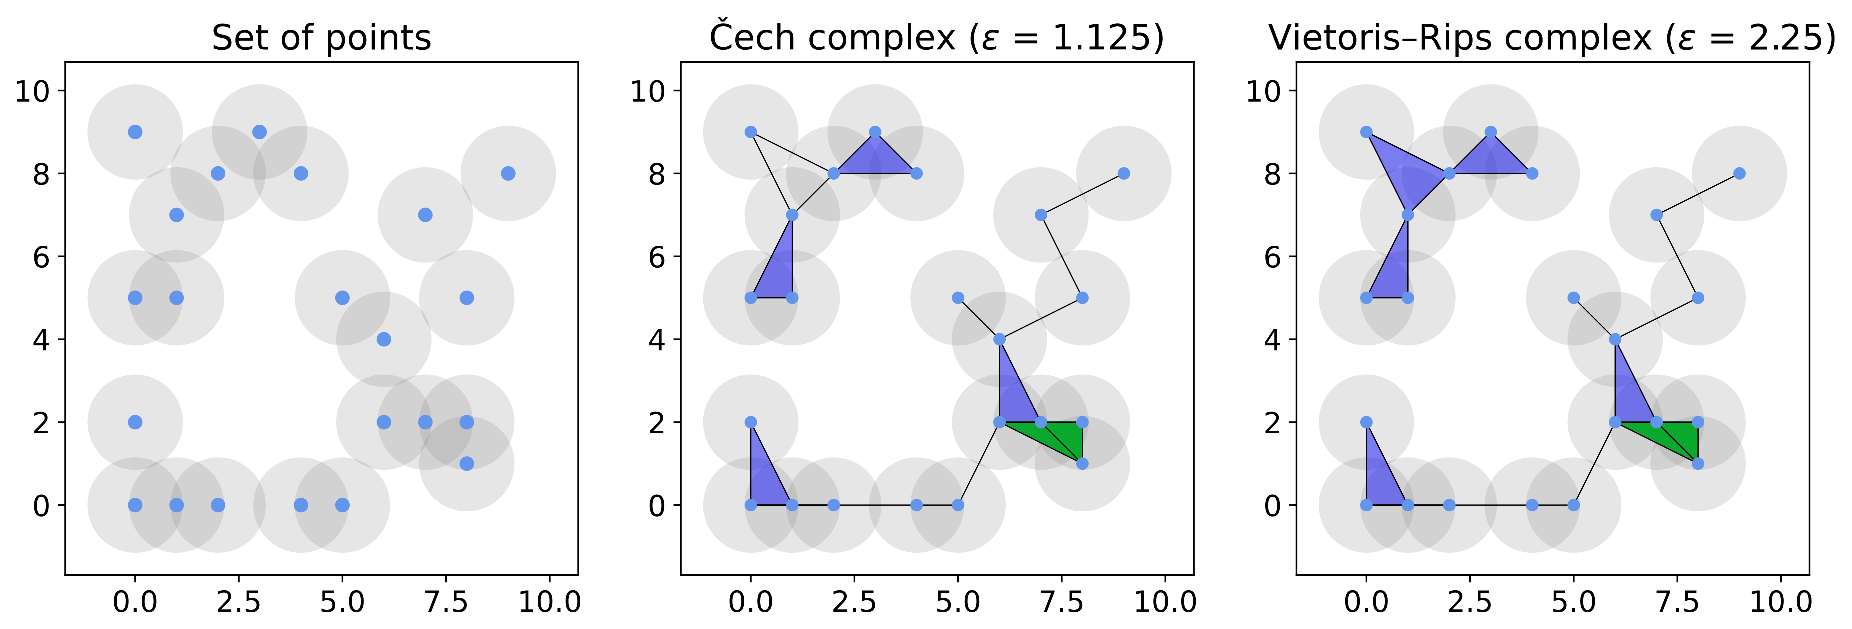
\includegraphics[width=\columnwidth]{figure2.eps}
            \caption{A synthetic point cloud with its \v{C}ech and Vietoris--Rips complexes for some values of the filtration parameter.}
            \label{figure2}
        \end{figure}\

    \item 
        Calculate the persistent homology of the resulting structure based on the `times' of appearance and disappearance of the simplices. Construct and filter (that is, remove the points closest to the diagonal, which carry little information and most likely describe the `noise' in the data) the persistence diagram, where each simplex corresponds to one point with coordinates along the `x' and `y' axes equal to the moments of its appearance in and disappearance from the complex, respectively.

    \item 
        Extract the features --- various topological and statistical characteristics --- from the persistence diagram. The principal approach studies Betti numbers~\cite{Zomorodian2005}, which represent the maximum number of cuts before separating the surface into two parts. One can also prove that the k-th Betti number equals the quantity of k-dimensional `holes' in the original metric space, which, in turn, is equivalent to the number of simplices of dimension k. Multiple other techniques have been proposed, including the persistence entropy~\cite{10.1007/978-3-319-29228-1_11}, landscape~\cite{bubenik2015statisticaltopologicaldataanalysis}, silhouette~\cite{chazal2013stochasticconvergencepersistencelandscapes}, and amplitude. The latter is particularly interesting as a measure of the difference between a given persistence diagram and an `empty' diagram, computed based on other topological characteristics as well as methods from adjacent fields of study~\cite{kerber2016geometryhelpscomparepersistence}, such as the Wasserstein~\cite{10.1145/62212.62253} and bottleneck distances~\cite{Efrat2001}. These features have proven effective for many classical machine learning algorithms to solve various problems.

    \item 
        Select the most valuable features and reduce the dimensionality of the obtained feature space to remove noise and improve the performance of machine learning algorithms applied later. For this, we used two predominant traditional techniques --- principal component analysis~\cite{Eckart_Young_1936} (PCA) and autoencoder~\cite{Autoencoder} (AE) --- as well as two topology-based methods --- uniform manifold approximation and projection~\cite{mcinnes2020umapuniformmanifoldapproximation} (UMAP) and representation topology divergence autoencoder~\cite{trofimov2023learningtopologypreservingdatarepresentations} (RTD AE).
\end{enumerate}

\section{Feature engineering}

As shown in \fref{figure3}, we employed three independent techniques to extract features from the EEG.\@

\begin{figure}
    \centering
    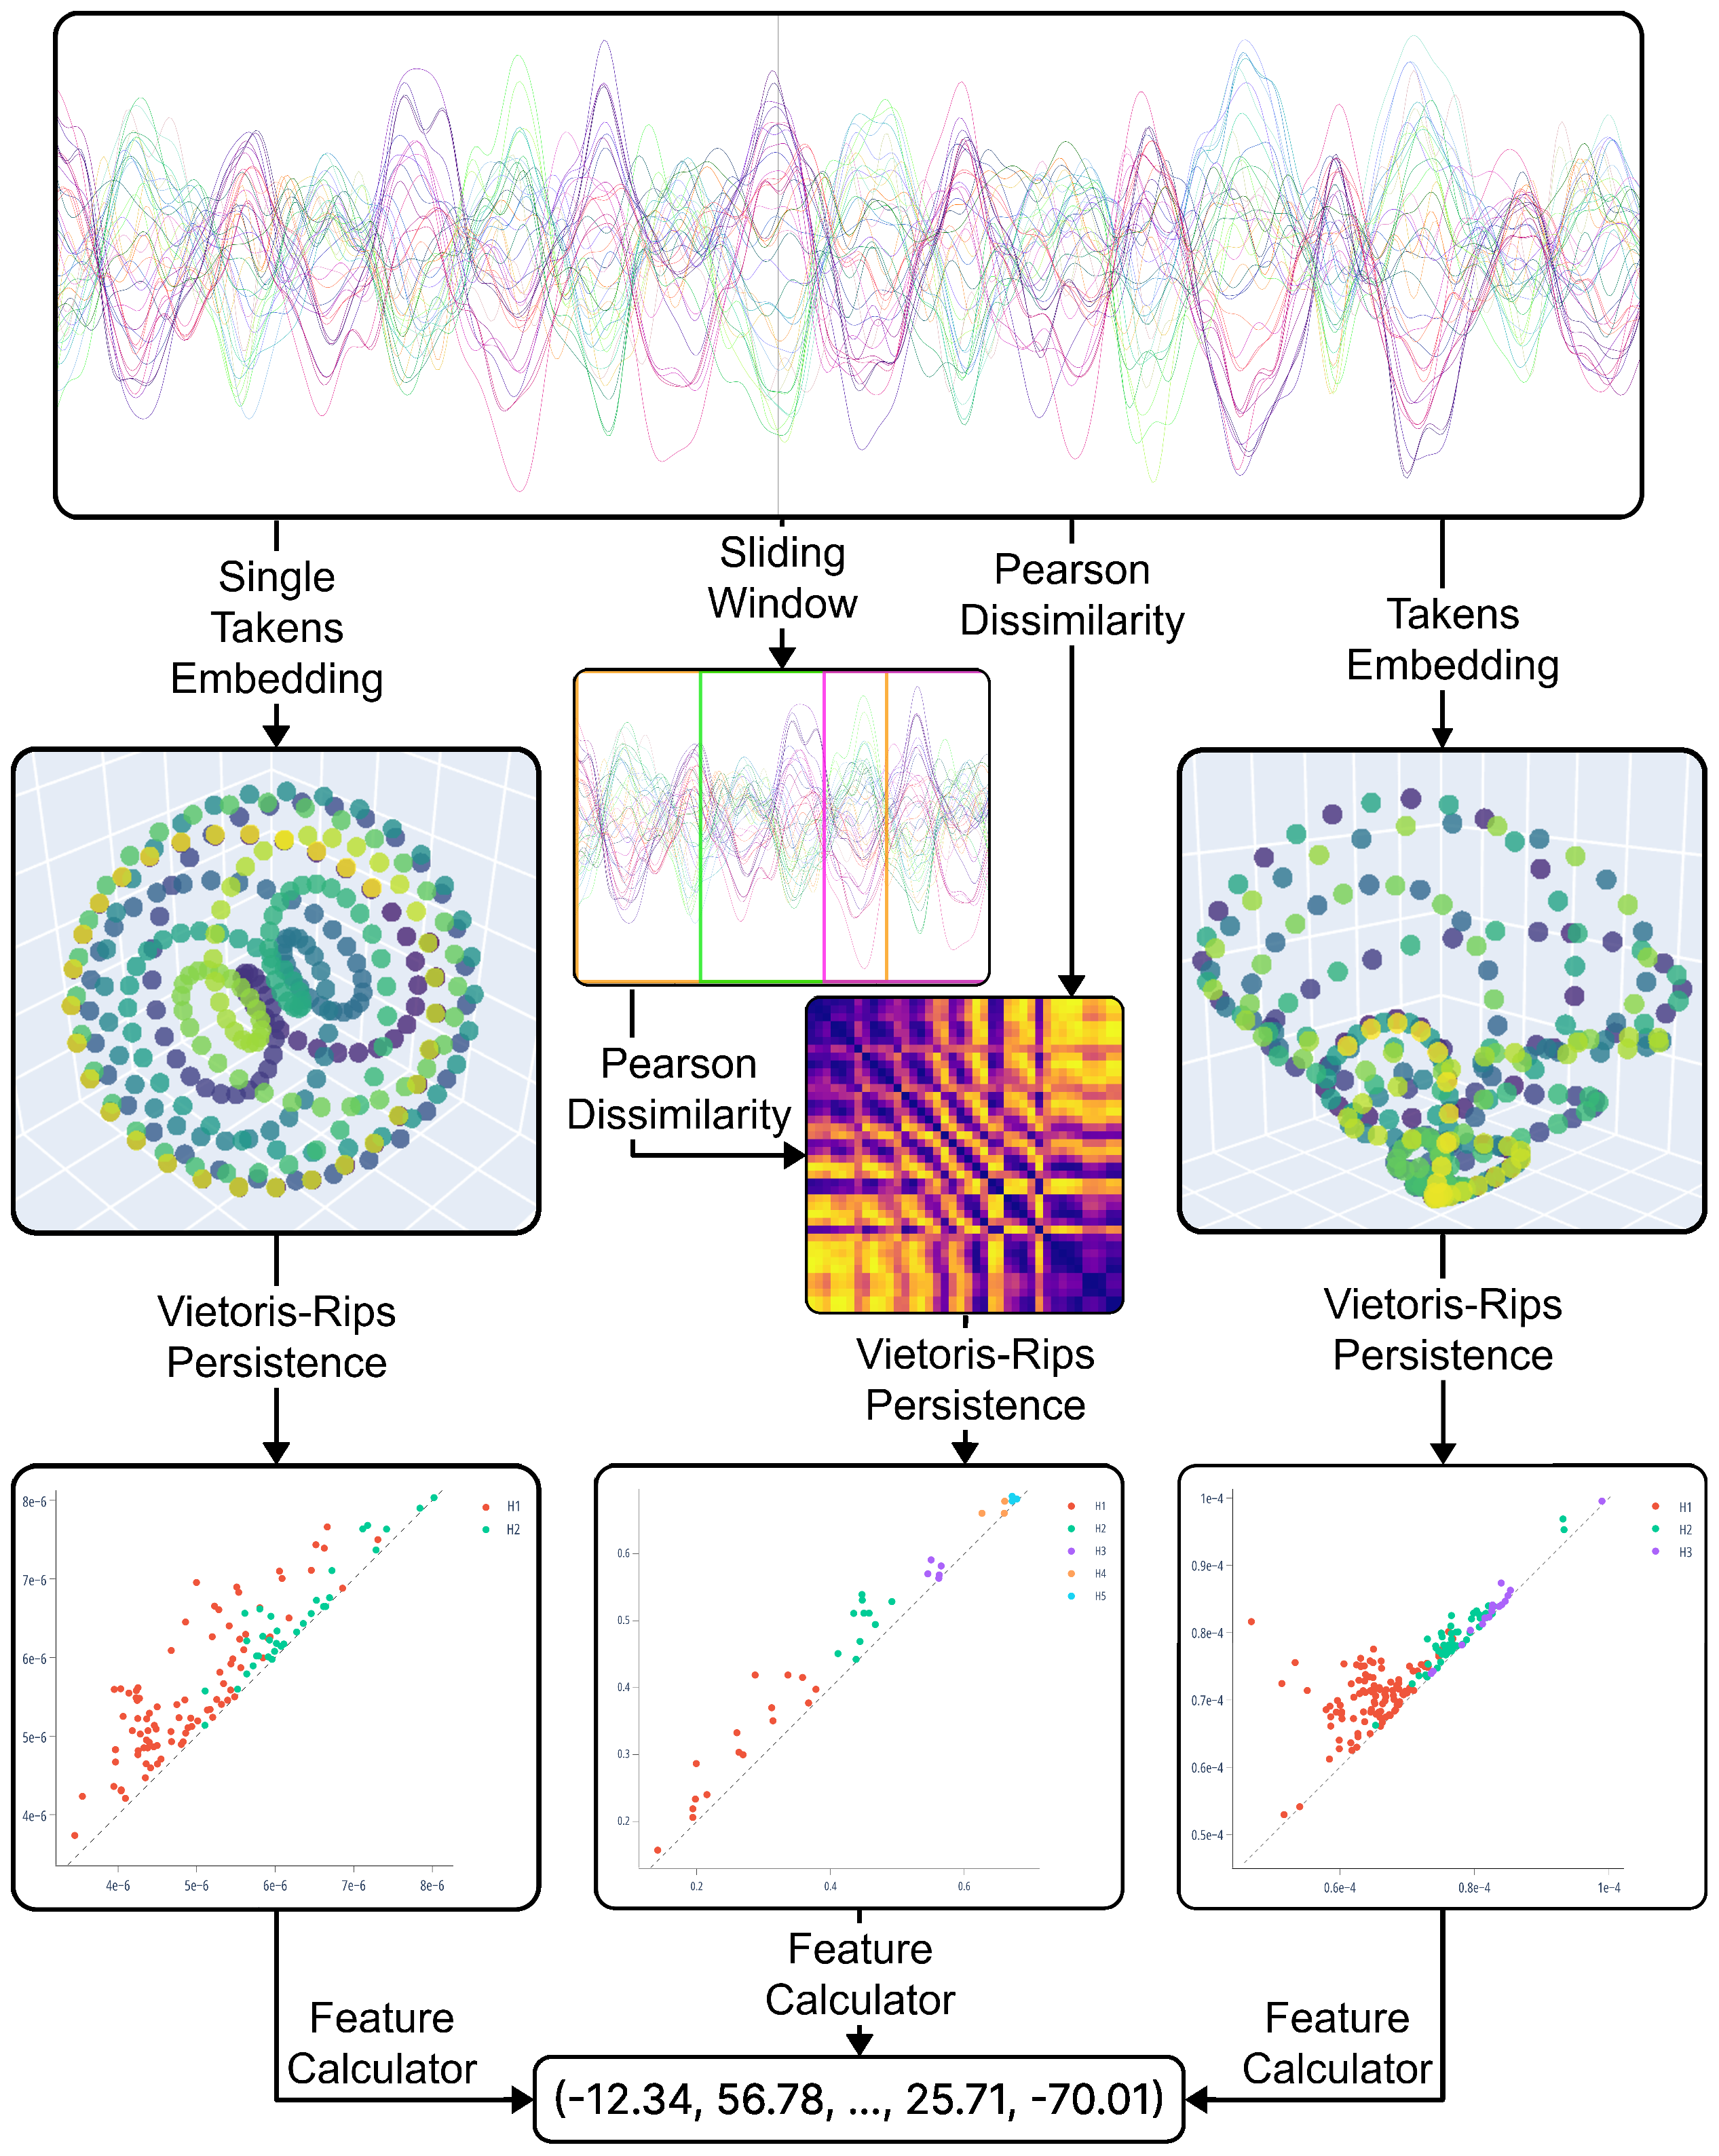
\includegraphics[width=\columnwidth]{figure3.eps}
    \caption{The scheme of the algorithm for extracting the topological features from the EEG.\@}
    \label{figure3}
\end{figure}

First, the EEG components are processed independently to analyze the records obtained at each electrode separately from the other parameters. For this, we divide the epochs --- multidimensional time series --- into sets of one-dimensional time series, each corresponding to one electrode during the experiment. Then, we calculate the optimal hyperparameters of the Takens embedding algorithm for each obtained time series. As a result, we acquire a set of hyperparameters for each epoch of each EEG component and select one value for each that is optimal for most epochs. Finally, we transform the original EEG into metric spaces using the Takens algorithm with the calculated best hyperparameters, construct Vietoris--Rips complexes, and compute persistence diagrams.

This approach describes individual EEG variables and detects most of the significant patterns in the data. However, it does not account for correlations between the components of the time series, which may contain the information necessary to solve the problem.

To address this issue, the second approach aims to analyze the relationships between the EEG components. The point clouds are obtained by calculating the Pearson dissimilarities between the channels for each epoch and all its sliding windows of a given size with a fixed step. The result is a set of matrices describing metric spaces consisting of as many points as the number of channels in the data, with distances reflecting the correlations between the corresponding components of the time series. Then, similar to other techniques, we apply Vietoris--Rips complexes to construct persistence diagrams and obtain the feature descriptions of the EEG.\@

Eventually, we analyze the time series as a whole without explicitly focusing on specific characteristics. To do this, we employ the multidimensional Takens embedding algorithm with hyperparameters determined experimentally but kept identical for all components. The retrieved metric spaces are again processed with Vietoris--Rips complexes to obtain the resulting features.

\subsection{Extracting features from persistence diagrams}

To vectorize the persistence diagrams as part of the feature engineering process, we implemented the pipeline shown in \fref{figure4}.

\begin{figure}
    \centering
    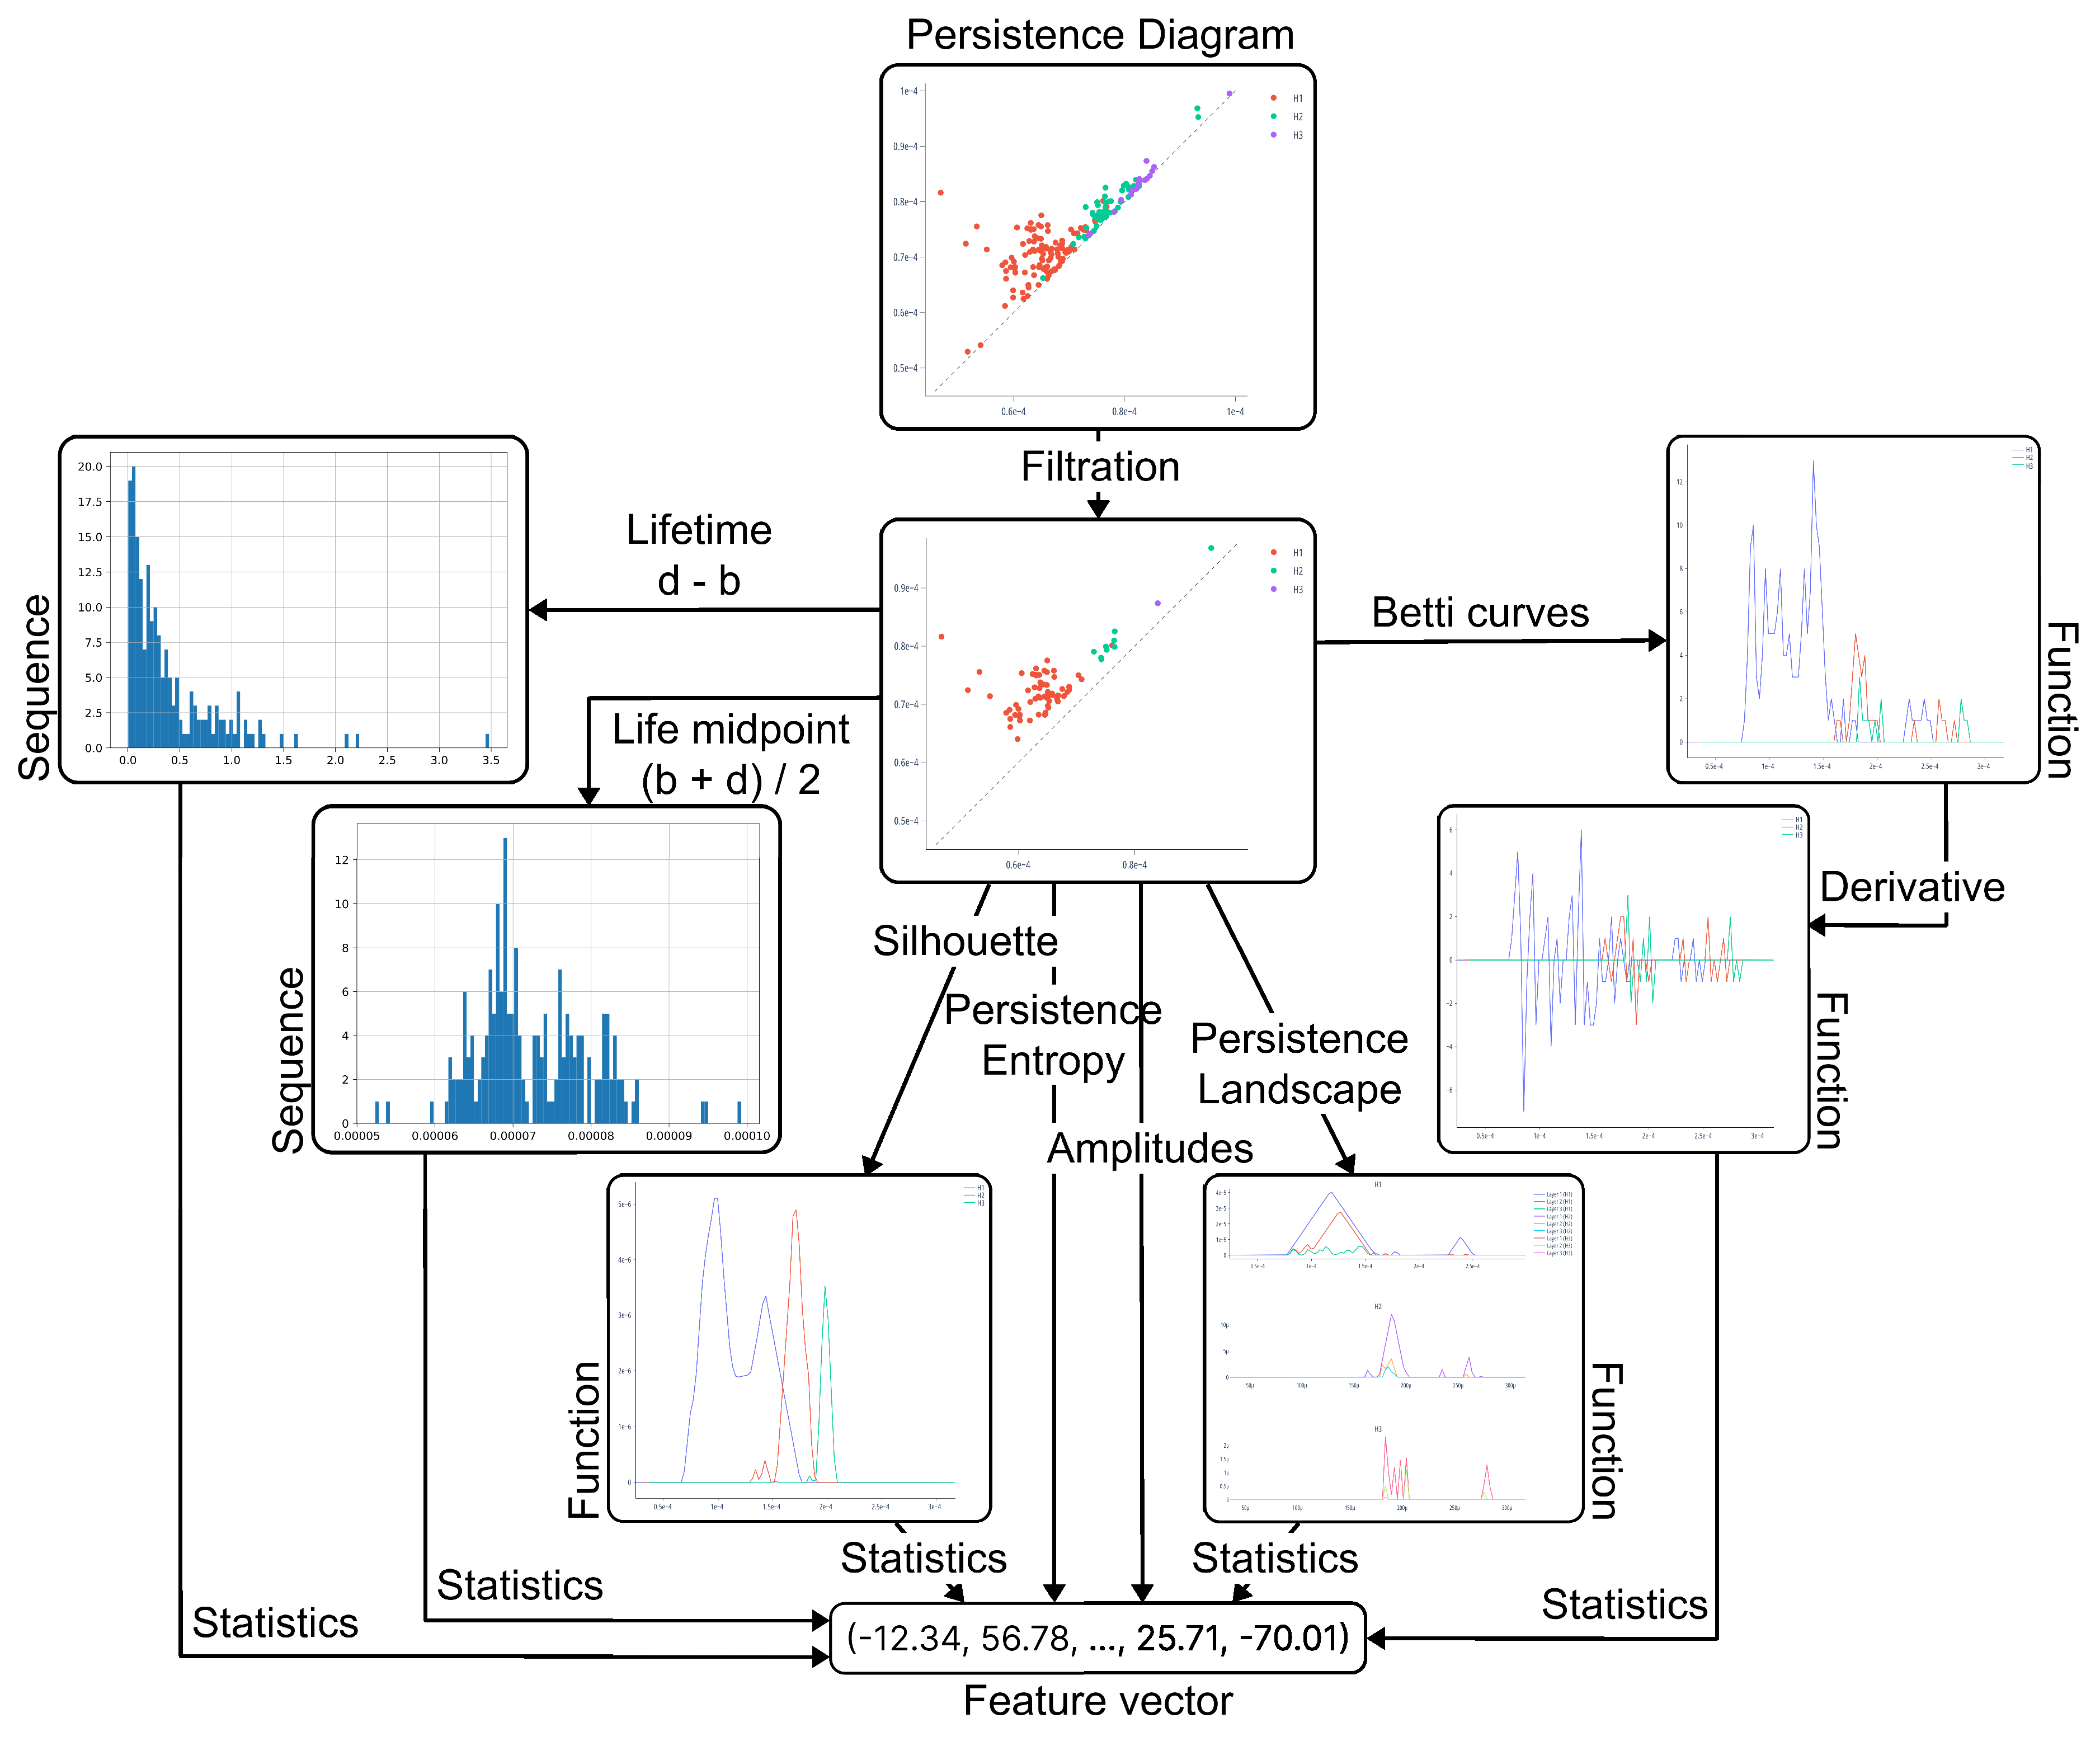
\includegraphics[width=\columnwidth]{figure4.eps}
    \caption{The scheme of the pipeline to vectorize the persistence diagrams.}
    \label{figure4}
\end{figure}

To improve the generalization ability of the features, the algorithm begins by filtering the persistence diagrams --- removing a fixed fraction of the points closest to the diagonal, hence representing the simplices with the shortest lifetimes. These usually carry little information and most likely describe the `noise' ---  the patterns present in the original data but not generic among the objects of interest. The remaining points, in turn, are the most `long-lived' simplices that disappear significantly later than they appear and are generally most interesting for the analysis. 

The algorithm then calculates various topological and statistical characteristics described previously to construct a comprehensive feature description of the persistence diagram. Specifically, it computes the following values:
\begin{itemize}
    \item 
        The statistical characteristics of the sequences of simplex lifetimes and of simplex life midpoints, of the first derivatives of Betti curves, of the first levels of persistence landscapes, and of the persistence silhouettes of degrees 1 and 2;
    \item 
        The persistence entropy;
    \item 
        Persistence amplitudes and their vector norms of the first and second orders using the bottleneck distance, the Wasserstein distance, the Betti curves, the persistence landscapes, and the persistence silhouettes.
\end{itemize}

By the statistical characteristics of a numeric sequence or a function, that is, of a random variable, we suggest the following values:

\begin{itemize}
    \item 
        The quantity, maximum, sum, mean, standard deviation, and various percentiles (25th, 50th, and 75th) of the elements;
    \item 
        The Manhattan and Euclidean norms of the input as a vector;
    \item 
        The skew and kurtosis of the variable, that is, the ratio of the third and fourth central moments to the cube and the fourth power of the standard deviation, respectively.
\end{itemize}

To avoid missing significant patterns, we performed all calculations not only for the entire persistence diagram but also for each simplex dimension individually. When calculating the statistical characteristics of the functions, we converted them into numeric sequences by selecting 100 values evenly over the interval of interest. Finally, we standardized all features to remove the scale factor from further decisions, which is known to improve the quality of most machine learning methods.

\subsection{Feature selection}

The feature engineering algorithm described earlier is designed to detect many patterns that may be present in the analyzed time series. However, this leads to an extremely high dimensionality of the resulting vectors, which is undesirable for most machine learning methods, including SDA, and may harm the quality of the final answer, especially if most assumed patterns are not present in the time series or appear insignificant to the target variable.

To address this issue, we introduce a quick state-detecting algorithm (QSDA) --- an additional step to select the most substantial features and filter out the noise that harms the final result. The algorithm operates as follows:
\begin{enumerate}
    \item 
        Calculate the possible final answers --- sets of state boundaries --- considering only one of the features by running a reduced SDA (that is, SDA with most hyperparameters adjusted to decrease the number of iterations, thus improving performance, without a significant loss in quality);
    \item
        For every produced set of edges, generate all possible ways to decrease the number of stages by merging the adjacent ones according to the rules provided by the SDA implementation as described previously;
    \item
        For every said way, calculate its quality as a multiple of the number of stages and the average silhouette coefficient against the considered feature over all pairs of adjacent stages. This allows us to focus on the most consistently valuable features and discard those that poorly detect many stages or perfectly distinguish only a few.
    \item 
        Consider the maximum of the values obtained in the previous step as the quality score of the feature;
    \item
        Repeat the process for all features and select those with the highest quality scores as the most informative.
\end{enumerate}

One may also apply additional heuristics to remove noisy, degenerate features, which are scored well solely because of the specifics of the approach. For example, consider a feature with only three non-zero values at indexes 300, 600, and 900 for an EEG of length 1200. In stages 1 -- 2 the algorithm might calculate the boundaries $\{ 0, 280, 320, 580, 620, 880, 920, 1200 \}$, which results in a $0.74$ average silhouette and a $5.93$ final quality score of the feature, putting it above most non-degenerate ones in stage 5. Although the feature may contain some relevant information, it is evidently not valuable and will harm the final result. To counteract this, we preemptively filter out all features with fewer than 200 unique values --- approximately 20\% of the length of the analyzed EEG.\@

\subsection{Information value analysis}

Information value analysis~\cite{InformationValue} is a typical approach to evaluate the influence of individual features on the target variable in binary classification problems and can be natively generalized to assess the importance of features for clusterization.

Suppose $x=(x_1, x_2, \ldots, x_n)$ is a categorical feature with values from the set $\{ X_1, X_2, \ldots, X_k \}$ and $y=(y_1, y_2, \ldots, y_n)$ is a binary target variable. Then, for each value $X_i$, the weight of evidence is calculated using equation \eref{eq2} as the ratio of the shares of positive and negative objects with this value of the feature. Finally, the information value of this feature is computed using equation \eref{eq3} and is an estimate of how much the distribution of this feature coincides with the distribution of the target variable, thus showing the importance of this feature for the correct classification of objects.

\begin{eqnarray}
    sharePos_i = numPos_i / numPos, \nonumber\\
    shareNeg_i = numNeg_i / numNeg, \nonumber\\
    WoE_i = ln(sharePos_i / shareNeg_i), \label{eq2}\\
    IV = \sum_{i = 1}^{k} (sharePos_i - shareNeg_i) \cdot WoE_i, \label{eq3}
\end{eqnarray}
with:
\begin{itemize}
    \item
        $numPos_i$ and $numNeg_i$ the numbers of objects belonging to the positive and negative classes, respectively, whose value of the feature is $X_i$;
    \item
        $numPos$ and $numNeg$ the total numbers of objects belonging to the positive and negative classes, respectively;
\end{itemize}

When working with quantitative features, the values are divided into several containers (we used 10) of the same length and processed as categorical based on their belonging to one or another container. For a multi-class classification problem, the information value is calculated independently for each class relative to a binary indicator variable with subsequent averaging of the values. The clusterization task is considered similarly, with each cluster treated as a separate class.

Large information values correspond to the high generalization ability of the feature and its significant influence on the correct prediction of the target variable. On the other hand, values close to zero indicate the harmfulness of the feature when making predictions.

\section{Results}

\subsection{Meditation data}

In this study, we primarily work with Guhyasamaja Tantra meditation data. First, we focus on subjects 1 -- 3 and compare the results obtained using 765 traditional features from~\cite{SDA}, almost 20000 topological features, a subset of 1500 -- 2000 topological features selected with QSDA, and the feature space with both approaches combined. At this stage, we determine the optimal hyperparameters, compare four dimensionality reduction algorithms, employ information value analysis, and study the scores calculated by the QSDA to select a set of approximately 4,000 topological features. The final hyperparameter values are listed in Supplementary Materials A. Then, we remove the characteristics that consistently show bad IV and QSDA quality from the computations and run the experiments for all 30 subjects to ensure the reliability of the results. To reinforce the stability of the approach, we also report the performance for Gaussian noise-corrupted recordings, expecting to see no significant changes in the detected stages, and shuffled EEG epochs, anticipating the detection of no good boundaries, resulting in close-to-zero quality metrics.

\subsubsection{Stage 1: full feature set for subjects~1 -- 3}

Based on the results shown in \fref{figure5}, the most stable and performant dimensionality reduction technique is PCA, which we thus used further throughout the experiment to reduce the feature spaces to 15 components  to improve comparability and filter out the noise, capturing only the most significant patterns. The features generated by UMAP demonstrate good clusterization quality independent of the number of components for all subjects but have relatively low explained variance, which greatly hinders their interpretability. On the other hand, the traditional autoencoder reflects the original feature space well and demonstrates quality similar to PCA.\@ However, for further calculations, as mentioned previously, we selected the latter, a more deterministic approach to speed up the computations and facilitate comparison with the original paper's results. Interestingly, the topological autoencoder produces mostly meaningless embeddings and has a low explained variance, while also achieving the worst results among all the methods. 

\begin{figure}
    \centering
    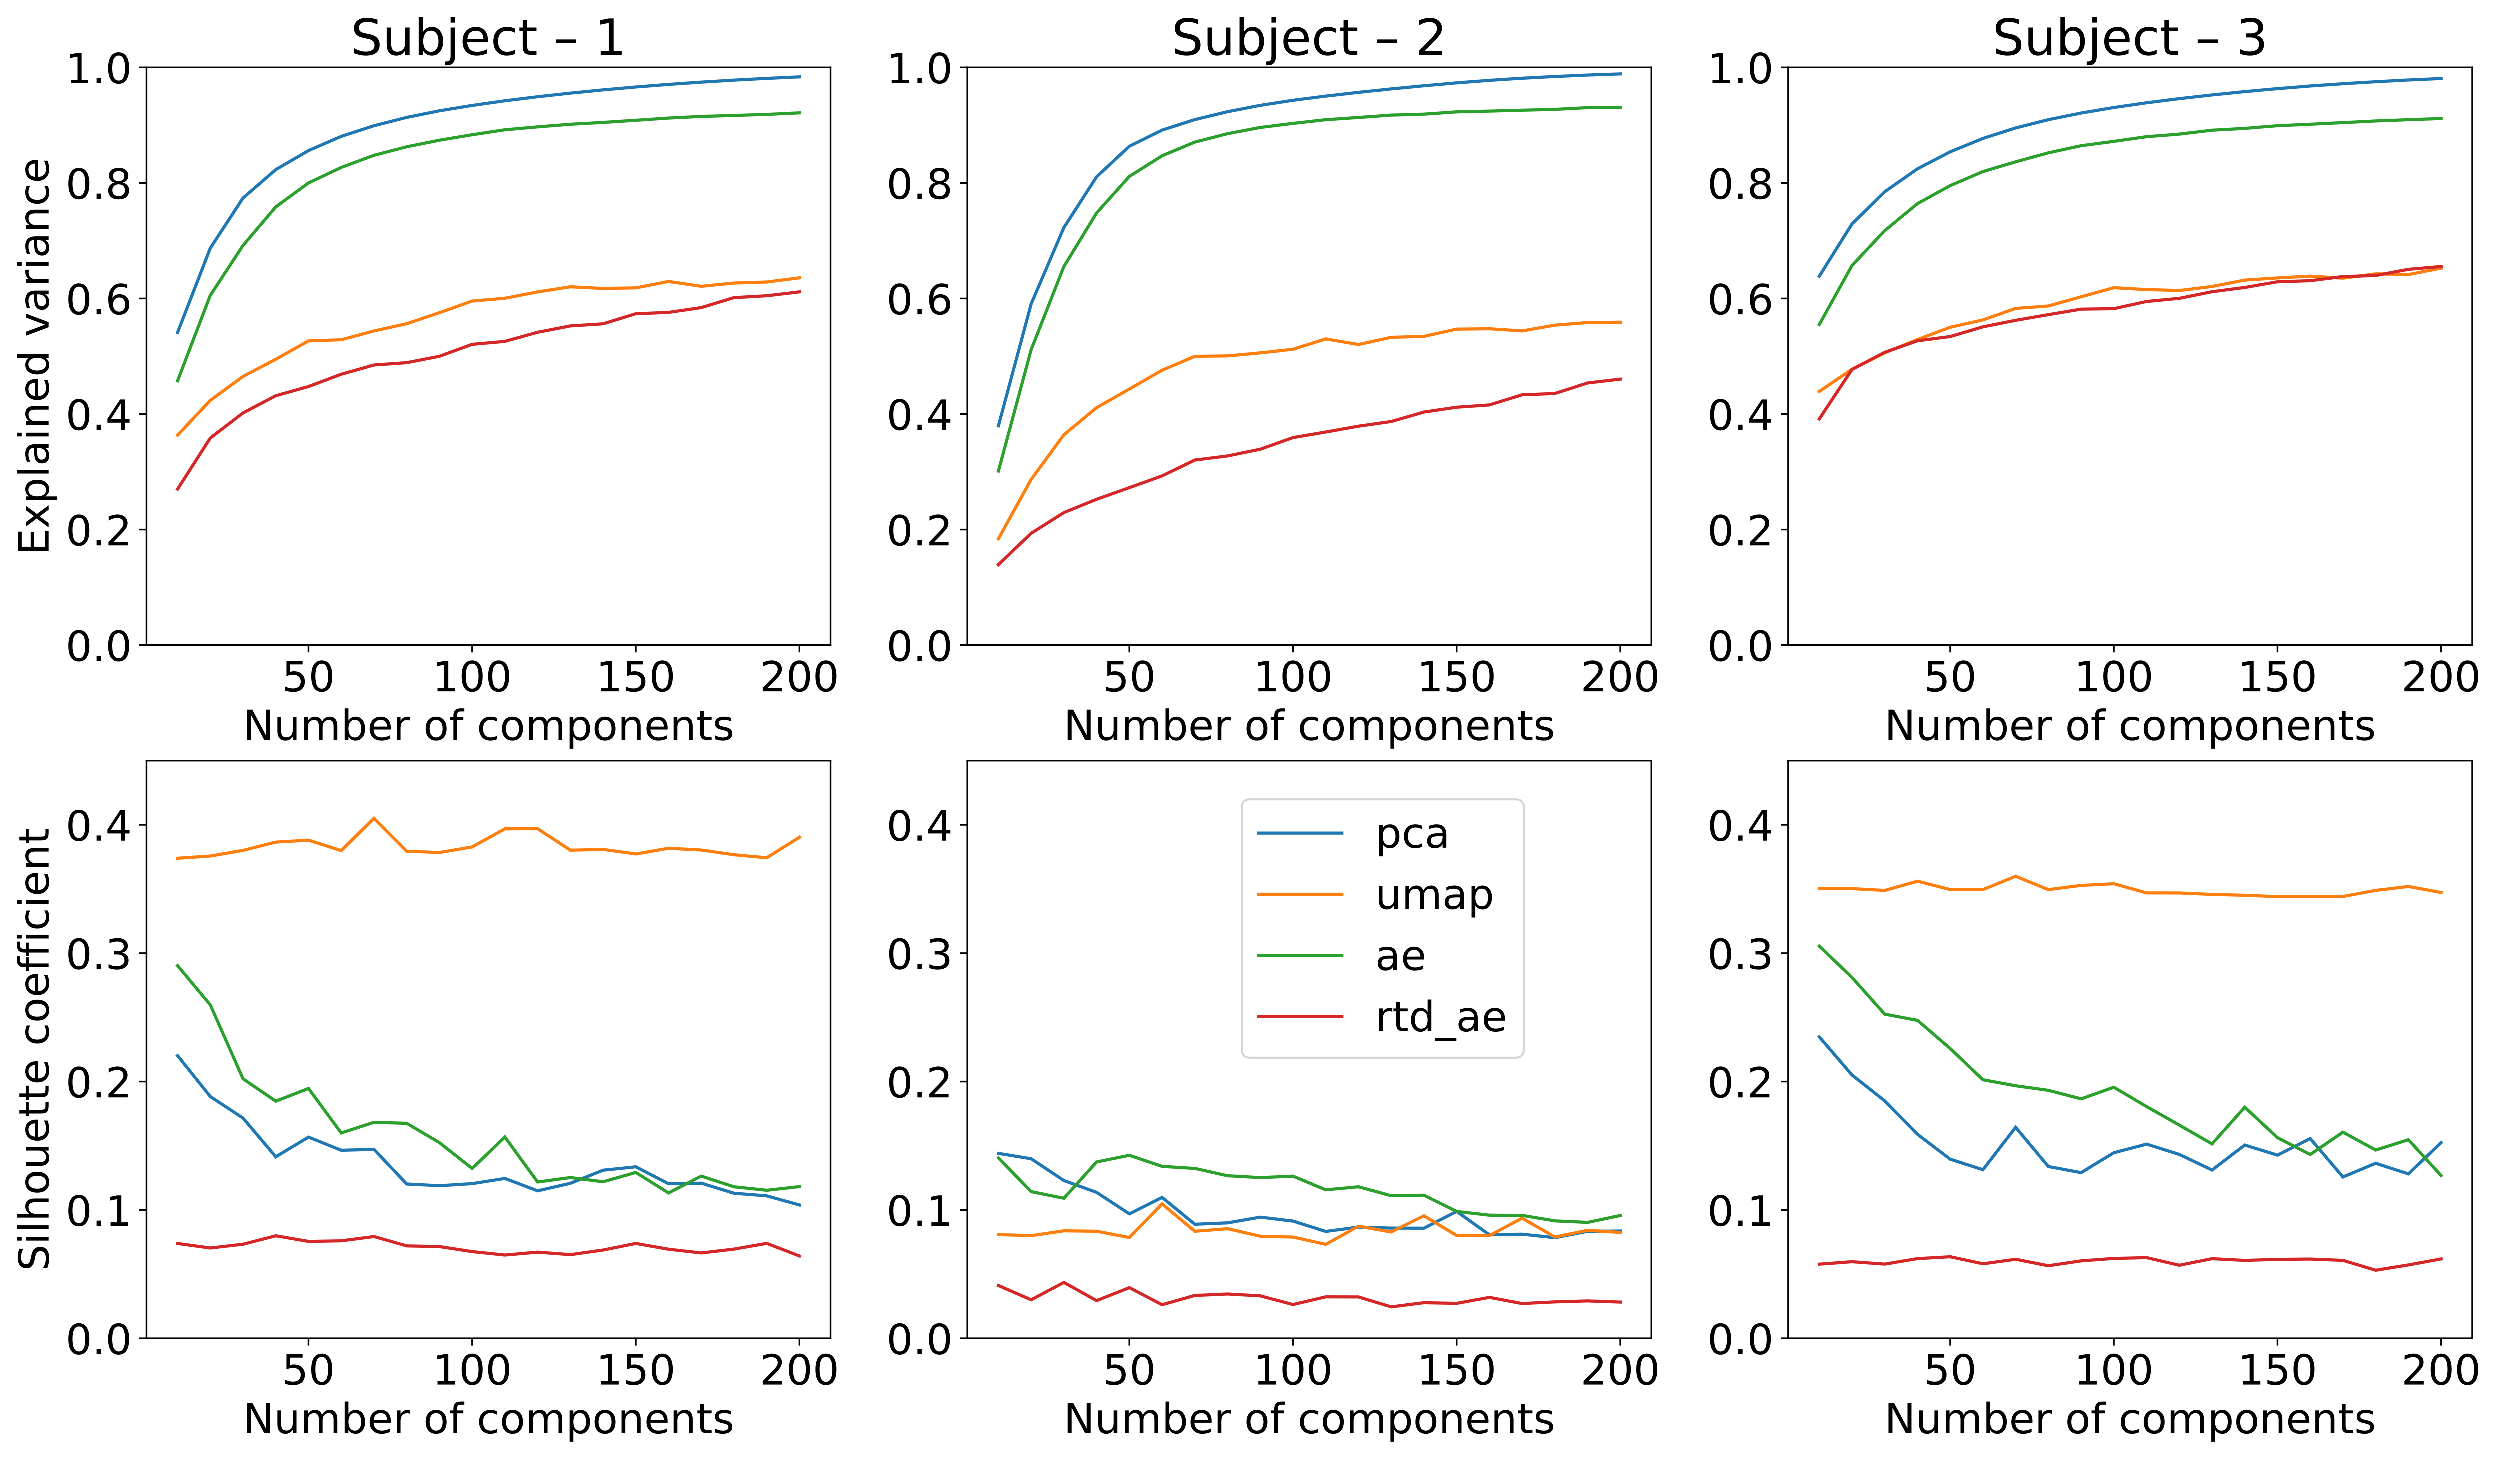
\includegraphics[width=\columnwidth]{figure5.eps}
    \caption{
        Explained variance (top) and achieved resulting quality (bottom) of four dimensionality reduction algorithms for subjects 1 (left), 2 (middle), and 3 (right).
    }
    \label{figure5}
\end{figure}

According to \tref{table1}, the filtered topological features outperform the traditional ones for all experiments, with the combined feature space achieving an even higher adapted silhouette score for subject 1, although following slightly behind for subjects 2 and 3. Notably, for all three subjects, the QSDA improved the quality of the resulting edges, indicating that the technique effectively filtered out noisy, harmful features. Finally, as expected, SDA revealed no significant patterns when applied to the shuffled recordings, demonstrating a quality more than 25 times lower than that of the original data. Nevertheless, adding Gaussian noise had a much smaller effect on the silhouette value, indicating that the pipeline is relatively robust with respect to noise.

\begin{table*}
    \caption{
        \label{table1}
        Adapted silhouette coefficients (that is, the average silhouette score of all pairs of adjacent stages) of results obtained from original, noisy, and shuffled recordings of subjects 1 -- 3 using different sets of features.
    }
    \begin{indented}
  \centering
    \item[]\begin{tabular}{@{}lllll}
    \br
    EEG recording & Traditional & Topological & Topological, QSDA & Combined\\
    \mr 
        Subject 1 (original)       & 0.198 & 0.126 & 0.205 & 0.218 \\
        Subject 1 (gaussian noise) & -     & -     & 0.056 & -     \\
        Subject 1 (shuffled)       & 0.004 & -     & 0.009 & 0.006 \\
    \bs
        Subject 2 (original)       & 0.110 & 0.051 & 0.131 & 0.126 \\
        Subject 2 (gaussian noise) & -     & -     & 0.048 & -     \\
        Subject 2 (shuffled)       & 0.008 & -     & 0.006 & 0.009 \\
    \bs
        Subject 3 (original)       & 0.111 & 0.105 & 0.190 & 0.187 \\
        Subject 3 (gaussian noise) & -     & -     & 0.099 & -     \\
        Subject 3 (shuffled)       & 0.017 & -     & 0.005 & 0.005 \\
     \br
    \end{tabular}
    \end{indented}
\end{table*}

Next, we review the specific results presented in Supplementary Materials B for each subject. Overall, the SDA successfully identified well-separated functional stages in all three EEG recordings for all the considered feature spaces. Although we did not achieve a complete agreement between the results, one can undoubtedly trace the common patterns confirmed by relatively good values of quality metrics for all subjects.

Most importantly, topological features demonstrated results comparable to those of traditional features, with some stage boundaries almost precisely matching for all types of features across all subjects. Furthermore, the topological approach led to better partitions, as measured by the silhouette coefficient, for all the monks. Traditional techniques, however, usually prevailed in terms of the stability of the answers: the scatter plots show noticeably higher density and better separation of the stage\mbox{-}2 boundary candidates when the spectral features are involved, except, arguably, for subject 2, where the illustrations are insufficient to make conclusive decisions.

With topological features, the algorithm significantly shifted or did not determine the individual boundaries separating similar states with low intercluster distances. This may indicate either that topological methods miss important patterns present in the original data, or that they reveal additional significant dependencies not recorded by the spectral features. Accounting for the results with the combined feature space, we suggest that the topological features most likely do not duplicate but complement the traditional ones to achieve even better, more stable results. Our experiments show that they may miss some critical patterns but discover other unexplored ones, reinforced by the combined features demonstrating comparable or better quality than other approaches while exhibiting higher stability. 

Finally, despite relatively low silhouette scores, the boundaries detected for noisy recordings mostly coincide with those for the original EEG, except for a few of the least stable ones. This reinforces the robustness of the topological approach.

Considering the feature quality scores presented to the right of each figure in Supplementary Materials B, the most practical features consistently across the QSDA and information value analysis for all subjects were various persistence amplitudes. Interestingly, QSDA primarily favored those based on persistence silhouettes and landscapes, while those calculated from betti curves received a higher IV.\@

Similarly, the QSDA and IV scores were generally consistent among the feature selection methods. For subject 1, both strategies valued recordings obtained from the right frontal and occipital parts of the brain; for subject 2, from the pre-frontal, frontal, and midline areas; and for subject 3, from the temporal and frontal brain regions. Notably, QSDA generally shifted its preference towards the occipital and parietal regions, although the principal trends persisted. However, neither technique revealed evident patterns in the brain regions producing the most valuable features that would be reliably observed for all subjects, indicating that no EEG channel should be excluded from further calculations. Regardless, both approaches consistently scored the features resulting from Pearson dissimilarities low.

Aggregated by topological origin, although the simplices of dimensions 1 and 2 contributed the most, the best features were those describing all dimensions simultaneously, suggesting that higher dimensions do not duplicate but rather complement the patterns detected by simpler features. Interestingly, for subject 2, the QSDA also favored simplices of dimension 5, which was not observed in other cases.

Finally, the most meaningful statistical characteristics, as suggested by the bar charts in Supplementary Materials B, were the vector norms with $p = 1$ and $p = 2$, as well as the sum and mean of the input. The least informative, in turn, were all percentiles (25, 50, and 75), skew, and kurtosis of variables.

It is worth noting that the extremely high dimensionality of the topological features may have introduced some dispersion in the results. However, the proposed selection method (QSDA) demonstrated effectiveness in filtering out significant portions of harmful features, supported by information value analysis. Although one may notice some discrepancies in its behavior compared to IV (for example, giving preference to the data collected closer to the occipital part of the brain and overestimating the quality of some amplitudes), the principal patterns match for both approaches.

\subsubsection{Stage 2: reduced feature set for all 30 subjects}

\begin{figure*}
    \centering
    
\includegraphics[width=\textwidth]{figure6.eps}
    \caption{The adapted silhouette scores of the resulting boundaries deduced by SDA using three types of features for the original and shuffled recordings of 30 subjects.}
    \label{figure6}
\end{figure*}

To speed up the subsequent computations and enhance the stability of the detected stages, we remove the consistently least effective features based on previous results:
\begin{itemize}
    \item 
        All features computed from Pearson dissimilarities between the components of the EEG;\@
    \item 
        Features resulting from the Betti curves and the number of points on the persistence diagrams, including the respective amplitudes;
    \item 
        The percentiles, skew, and kurtosis of the variables.
\end{itemize}
By doing this, we reduce the topological feature space to approximately 4,500 features (as opposed to 20,000 previously), from which we select the 25\% best ones using QSDA. Moving forward, we repeat all the experiments for 30 subjects and report the results in Supplementary Materials C.

First, based on the silhouette scores presented in Supplementary Materials C, Table 1, and the aggregated illustration in \fref{figure6}, the topological features outperform the traditional ones for most subjects, with the combined feature spaces prevalent in a third of the recordings. Similar to previous findings, QSDA improves the results for almost all subjects, reinforcing its effectiveness in feature selection. Furthermore, Gaussian noise generally reduces the score by at most a factor of three, while shuffling the epochs drastically decreases the quality, indicating no good boundaries to be detected. Indeed, the scores in the latter case were multiple times lower than those for the original EEG and did not exceed 0.05 for most subjects. 

Exploring the detected stage boundaries also confirms our previous conclusions that all feature sets detect similar boundaries, with only the least stable ones noticeably shifted by the topological approach. Interestingly, unlike previously, the clusters derived from topological features appeared quite dense for most subjects, suggesting that the new approach is also not inferior in terms of the stability of the results. Moreover, for a significant portion of the subjects, the combined features produced more compact clusters than all other techniques, confirming that the two feature sets not only support each other but may also detect different meaningful characteristics of the EEG.

Finally, these experiments confirm which features are the most valuable for the study. As shown on the right of each figure in Supplementary Materials C, similar to the first three subjects, the most useful features were the amplitudes, especially those based on persistence silhouettes, with the mean and sum being the most practical characteristics to consider. Interestingly, the most valuable data for the research generally comes from the electrodes in the frontal area of the brain, as confirmed by both the aggregated QSDA and IV scores in \fref{figure7}. However, this result is not consistent across all subjects, with some exhibiting opposite tendencies, which requires further research into more specific physiological patterns of individual subjects.

\begin{figure}
    \centering
    
\includegraphics[width=\columnwidth]{figure7.eps}
    \caption{Feature quality scores (QSDA on the left, IV on the right) aggregated by their source electrode averaged over 30 subjects. To account for the distinctions in electrode placement during different expeditions, we merge similar electrodes from different recordings into one point on the diagram. The respective mappings are indicated in the labels of such points using the `/' symbol.}
    \label{figure7}
\end{figure}

Overall, the results with the full dataset confirm most patterns observed previously using the EEG of subjects 1 - 3. Although some stages have shifted when using topological features compared to the traditional approach, general trends persist, and the method is confirmed to be robust based on its performance with noisy and shuffled recordings. Furthermore, the proposed feature selection technique demonstrated promising results, noticeably boosting the final quality and being consistent with the information value analysis. Although further research is needed to evaluate the physiological interpretation of the conclusions and to understand the reasons for the observed discrepancies, the results obtained for the meditation data are promising and robust enough to consider the proposed topological framework as an appropriate alternative to traditional spectral features.

\subsection{Sleep data}

To reinforce our results and assess the applicability of the topological approach to other data, we run the proposed algorithm on PSG recordings from the sleep-edf dataset. As mentioned in Section 2.2, we use SDA to search for 10 functional stages and evaluate whether they fit any subset of expert annotations. For simplicity, this section analyzes three sets of features: spectral features similar to those in \cite{SDA}, topological features as described in Section 6.1.2, and a combination of both. Moreover, as the data contains only seven data channels, we omit the feature selection with QSDA to speed up the computations. All the hyperparameters of the algorithm were left unchanged.

To assess the results, we focus on two primary quality metrics: the previously used adapted silhouette coefficient and the Fowlkes-Mallows index (FMI)~\cite{Fowlkes01091983}. The latter is a typical external criterion used to measure the degree of similarity between two clusterings. For a predicted set of stage boundaries $A = (a_1, a_2, \dots, a_n)$ and an expert annotation $E = (e_1, e_2, \dots, e_m)$, we first select a subset $F = (f_1, f_2, \dots, f_n) \subset E$ of boundaries with the lowest sum of pairwise distances to A, as denoted by equation \eref{eq4}.
\begin{equation}
    \sum_{i = 1}^{n} |a_i - f_i| \rightarrow \min \label{eq4}
\end{equation}
Then, for each pair of epochs, we determine whether their `true' cluster distribution matches the predicted one, and compute the FMI according to equation \eref{eq5}.
\begin{equation}
    FMI = \sqrt{\frac{TP}{TP + FP} \cdot \frac{TP}{TP + FN}} \label{eq5}
\end{equation}
with:
\begin{itemize}
    \item
        $TP$ the number of pairs of epochs assigned to the same cluster in both distributions;
    \item
        $FP$ the number of pairs of epochs assigned to the same cluster in the `true' distribution, but to different clusters in the predicted one;
    \item
        $FN$ the number of pairs of epochs assigned to the same cluster in the predicted distribution, but to different clusters in the `true' one.
\end{itemize}

Interestingly, based on the results shown in \tref{table2}, the topological approach is noticeably superior to the traditional features for this data in both the silhouette coefficient and the Fowlkes-Mallows index. Moreover, a similar or even slightly worse quality obtained with the combined feature space suggests that for these data, the topological approach supersedes the traditional features, revealing not only new patterns but also supporting the already known ones.

\Table{
    \label{table2}
    Mean quality metrics and their 95\% confidence intervals of results for sleep data of 153 subjects obtained using three sets of features.
}
    \br
    Feature set & Adapted silhouette & Fowlkes-Mallows index \\
    \mr
    Traditional & $0.03 \pm 0.009$  & $0.843 \pm 0.017$ \\
    Topological & $0.228 \pm 0.01 $ & $0.911 \pm 0.013$ \\
    Combined &  $0.227 \pm 0.01 $ & $0.907 \pm 0.014$ \\
    \br
\endTable

Next, we present the comprehensive results separately for each subject in Supplementary Materials D. The figures suggest that all feature sets generally detect similar stages. Notably, the final boundaries typically fall within tight groups of expert labels, indicating that the algorithm effectively finds high-level clusterings, and the limitation of 10 searched stages does not impact the interpretability of the results. Moreover, as suggested by the densities of the scatter plots, topological features produce significantly more robust results, which at the same time better correspond to target labelings. The quality score diagrams at the beginning of Supplementary Materials D also support the findings that traditional features consistently perform worse than the topological approach in terms of both stability and agreement with target answers for almost all subjects.

Overall, the results for sleep-edf reflect previous findings from the meditation data but strongly suggest the superiority of the topological approach. Despite the constraint of searching for only ten stages, our experiments show that with topological features, SDA consistently produces more robust boundaries that better match the target distribution, even without feature selection techniques, including QSDA.\@

\subsection{A note on computational complexity}

Considering the large size of the topological feature space, it is essential to assess whether the gains in the quality of the final answer justify the computational expenses of generating almost 20000 features. Since estimating the theoretical algorithmic complexity for such an elaborate pipeline is infeasible, we resort to an empirical analysis of the methods' running times using samples from both datasets ranging from 50 to 500 epochs. For the experiments, we used a 16-core Intel Core i5-12600K CPU with 32GB of RAM powered by Windows. Each metric was calculated as the average of 25 measurements. The size of the 95\% confidence intervals for each entry did not exceed 1\% of their absolute value, so they are not presented further.

As shown in \fref{figure8}, calculating the topological features is indeed more expensive than the traditional ones for both datasets. However, the difference is not as significant as one might expect, and the topological approach may have high potential for optimization in the future, given the novelty of TDA and the numerous ongoing research projects published nowadays. Therefore, the suggested framework is a practical alternative to traditional spectral features, showing similar and, arguably, even better results with reasonable losses in computational efficiency.

\begin{figure}
    \centering
    
\includegraphics[width=\columnwidth]{figure8.eps}
    \caption{The running time of calculating traditional and topological features for two types of data, depending on the number of epochs.}
    \label{figure8}
\end{figure}


\section{Conslusions and discussion}

In this study, we explored a novel technique based on topological data analysis to construct comprehensive feature descriptions of time series. The algorithm proved to be an effective feature engineering approach for SDA, a recently introduced automated method for finding functional stages in a time series. As demonstrated by our experiments with 30 EEG recordings of the Guhyasamaja Tantra meditation practice and 153 PSG recordings of human sleep, using topological features, SDA detects boundaries similar to, and sometimes even superior in quality to, those obtained previously using solely spectral features. Most importantly, SDA produced particularly promising results for the sleep-edf dataset, where the boundaries detected based on topological features appeared noticeably more consistent with expert annotations for most subjects. Moreover, adding Gaussian noise to the original data did not fundamentally change the final results, and reduced the silhouette score by only a few times. However, When applied to shuffled epochs, SDA produced no reasonable stage boundaries with several times lower quality metrics compared to the original EEG for all analyzed objects. Thus, we consider the obtained results reliable and suggest that the topological approach is a trustworthy alternative to traditional methods, which produces good features and does not hinder the stability of the SDA.\@

However, in some cases, the technique favored less similar results, indicating both the loss of important information in the topological features and the discovery of new patterns previously not identified by existing solutions. Based on our research on the separate and combined behavior of traditional and topological features, we suggest that neither approach extracts a complete description of EEG in the general case. Although there are substantial intersections, topological and spectral characteristics typically focus on distinct patterns in the data, complementing each other to highlight known patterns and reveal new ones. Thus, there is no silver bullet to solve the task, but one should combine the approaches to achieve a robust result that reflects the actual behavior of the studied process.

Finally, we introduced QSDA, a new SDA-based feature selection framework that accounts for the specifics of the final task and scales well with large feature sets. As confirmed by our experiments using meditation data, QSDA is an effective technique for removing noisy, degenerate features that are detrimental to good clusterization of the EEG. The algorithm's scores primarily correlate with the information values of the features, which reinforces its results and supports the rationality of using the alleged best features to solve the problem at hand. Furthermore, using the QSDA, we successfully identified that the most valuable features for clustering Guhyasamaja Tantra meditation data generally come from sensors in the frontal areas of the brain. Although we do not currently have an explanation for this phenomenon, it may be an interesting observation worthy of consideration by physiological experts.

Future studies should test the proposed approach with other data sets to collect more examples, generalize the technique, and identify common patterns. We expect especially intriguing results when applied to well-studied data with a known correct placement of functional state boundaries. Moreover, we anticipate significant outcomes from studies aimed at interpreting the patterns recorded by topological features accounting for the structure and relations authentically observed in the original data from a physiological perspective.

\section*{Data availability statement}

The raw data will be made available by the authors upon request, without undue reservation.

\section*{Ethics statement}

The studies involving humans were approved by Moscow State University. The studies were conducted in accordance with local legislation and institutional requirements. All participants provided written informed consent to participate in this study.

\section*{Declaration of conflicting interest}

The author(s) declare no potential conflicts of interest with respect to the research, authorship, and/or publication of this article.

\section*{Acknowledgment}

This study was supported by the Russian Science Foundation, Grant No. 24-68-00030.

\section*{References}

\bibliography{references}{}
\bibliographystyle{iopart-num}

\end{document}
